%%%%%%%%%%%%%%%%%%%%%%%%%%%%%%%%%%%%%%%%%%%%%%%%%%%%%%%%%%%%%%%%%%%%%%%%%%%%%%%
% Dynamic Point Theory - Self-contained Nature-style manuscript
% Title: The Nature and Interior of the Mathematical Point,
%        and the Transition from Point to Consciousness
% Author: Xiaohui Li
% All figures are generated inline via TikZ/pgfplots; no external files needed.
%%%%%%%%%%%%%%%%%%%%%%%%%%%%%%%%%%%%%%%%%%%%%%%%%%%%%%%%%%%%%%%%%%%%%%%%%%%%%%%

\documentclass[11pt,a4paper]{article}

\usepackage[utf8]{inputenc}
\usepackage[T1]{fontenc}
\usepackage{geometry}
\geometry{left=2.5cm,right=2.5cm,top=2.5cm,bottom=2.5cm}

\usepackage{amsmath,amssymb,amsthm}
\usepackage{booktabs}
\usepackage[numbers,sort&compress]{natbib}
\usepackage{hyperref}
\usepackage{xcolor}

% --- Inline figure generation ------------------------------------------------
\usepackage{tikz}
\usepackage{pgfplots}
\pgfplotsset{compat=1.18}
\usetikzlibrary{shapes,positioning,calc}
% -----------------------------------------------------------------------------

\usepackage{caption}
\usepackage{subcaption}

\theoremstyle{definition}
\newtheorem{proposition}{Proposition}

\title{\textbf{The Nature and Interior of the Mathematical Point,\\ and the Transition from Point to Consciousness}}
\author{Xiaohui Li\\
\textit{Independent Researcher, Baoji, China}\\
\textit{Correspondence: danceluck@163.com}\\
\textit{ORCID: 0009-0003-8233-7191}\\
\textit{Data homepage: \url{https://github.com/xiaohui-li-lab/}}}
\date{}

\begin{document}

\maketitle

\begin{abstract}
\noindent
The mathematical point is traditionally defined as a geometric object without parts and without interior. Yet, when the temporal dimension and the process of dynamic generation are introduced into the foundations of mathematics, the static definition of the point faces a fundamental tension. Here we propose the \textit{Dynamic Point Theory} (DPT): if a mathematical point is to be identified and measured in the physical world, it must carry a conceptual-consciousness structure and therefore possesses a non-trivial interior; this interior can be modeled as a finite or infinite-dimensional subspace of a Hilbert space. Consequently, the mathematical point, the physical singularity, and consciousness are logically co-original. We further argue that the Big-Bang singularity and the singularity formed by stellar collapse are not of the same category; the former is a ``consciousness-mathematical point'' with an interior, whereas the latter is a cutoff of classical general relativity in the quantum-gravity regime. We provide formal propositions, Planck-scale boundary conditions, numerical simulations, and several testable predictions.
\end{abstract}

\noindent\textbf{Keywords:} mathematical point; Hilbert space; consciousness; singularity; black hole; Big Bang; quantum gravity; dynamic mathematics

\section{Introduction}

Euclid's \textit{Elements} defines a point as ``that which has no part'' \cite{euclid_elements}. This static definition has supported geometry for more than two millennia, but it now confronts challenges from modern physics: the black-hole singularities predicted by general relativity and the initial singularity assumed by the standard cosmological model are both described as point-like structures of vanishing volume and infinite density \cite{hawking_penrose1966, penrose1965}. However, the formation of a black hole from stellar collapse is a dynamical event---a supernova explosion produces both outward and inward forces; we observe the outward explosion, but we do not directly ``see'' the generation of a singularity \cite{woosley_janka2005}. Thus fact and theory diverge here: is the singularity a physical reality, or merely an extrapolation of mathematical idealization?

Mathematicians usually do not rashly identify a mathematical point with a physical singularity. We claim that no smooth transition exists between the mathematical point and the cosmological singularity; their relationship must be re-examined within a framework of ``dynamic mathematics''. We propose and prove a central proposition: if a point is admitted to be generated in time (the formation of a line being understood as the motion of a point), then a point cannot be a pure limit without interior; its interior can be characterized by a Hilbert space.

\section{Dynamic Mathematics and the Generation of Points}

\subsection{From the static point to the dynamic point}

In the classical definition the point precedes the line, the surface, and the solid. Yet human intuition of the line arises from the motion of a point, and intuitions of surface and volume arise from the motions of line and surface \cite{klein1939}. Therefore line, surface, and volume are essentially dynamically generated. If we reverse the question and ask ``what is a point?'', we must start from the generative process: the point is the smallest unit capable of initiating motion. We call such a point, identified through motion, a \textit{dynamic point}.

\subsection{Formal propositions}

\begin{proposition}[Interior existence of a dynamic point]
Let $P$ be a dynamic point whose state is described by a set of observable generative parameters
\begin{equation}
\Psi(P) = \{x_i(t), p_i(t), I_i(t)\}_{i=1}^{n},
\end{equation}
where $x_i$ are spatial coordinates, $p_i$ are momenta/generative directions, and $I_i$ are conceptual-informational loads. If $P$ is identifiable in any reference frame, then $\Psi(P)$ spans a non-zero Hilbert space $\mathcal{H}_P$ with $\dim(\mathcal{H}_P) \ge 1$. Hence $P$ has an interior structure.
\end{proposition}

\noindent\textit{Proof sketch.} If $\dim(\mathcal{H}_P)=0$, then $\Psi(P)$ would be empty and $P$ could not be identified by any measurement or conceptual operation; it would be indistinguishable from nothingness. By the observable postulate of quantum mechanics, any identifiable physical object corresponds to a non-zero vector in a Hilbert space \cite{von_neumann1955}. Therefore an identifiable point must have an interior. \hfill$\square$

\begin{proposition}[Planck boundary of a point]
Let $\delta x$ be the spatial extension of a dynamic point. If
\begin{equation}
\delta x < l_P = \sqrt{\frac{\hbar G}{c^3}} \approx 1.616 \times 10^{-35}\,\text{m},
\end{equation}
then the internal degrees of freedom of the point can no longer be described by classical continuous geometry and must be described by a quantum-gravity theory. The dimension of the internal Hilbert space then diverges or tends to a Planck cutoff value.
\end{proposition}

\subsection{Connection with the uncertainty principle}

A ``pure mathematical point'' would require simultaneous determination of position and momentum, violating the Heisenberg uncertainty relation \cite{heisenberg1927}. Therefore any realizable point must possess a finite extension; this extension is precisely its interior. The uncertainty principle thus becomes the physical guarantee that a point has an interior.

\section{The Interior of a Point as a Hilbert Space}

\subsection{The infinite within the infinitesimal}

Classical thought opposes the infinitely large to the infinitely small. We propose that at sufficiently small scales the infinitesimal can accommodate a Hilbert-space structure of ``infinite'' richness. This is consonant with the fractal-geometric spirit that the local contains the global \cite{mandelbrot1982}. We model the interior of a point as
\begin{equation}
\mathcal{H}_P = \bigoplus_{k=1}^{N} \mathcal{H}_k,
\end{equation}
where $N$ may be finite or divergent. Each $\mathcal{H}_k$ represents an internal degree of freedom: spin, flavor, color, conceptual bit, etc.

\subsection{Numerical simulation: scaling of the internal Hilbert-space dimension}

We construct a simplified model: let $\delta$ be the spatial extension of a point, and let the internal Hilbert-space dimension $D$ satisfy
\begin{equation}
D(\delta) =
\begin{cases}
D_0 \left(\dfrac{l_P}{\delta}\right)^{\alpha}, & \delta \ge l_P,\\[6pt]
D_0, & \delta < l_P,
\end{cases}
\end{equation}
with $\alpha \approx 2$ corresponding to two-dimensional phase-space quantization. Figure~\ref{fig:dim_scaling} shows $D(\delta)$ as a function of $\delta/l_P$. As $\delta$ approaches the Planck length, $D$ grows rapidly, suggesting that a singularity can harbor a large number of degrees of freedom.

\begin{figure}[htbp]
\centering
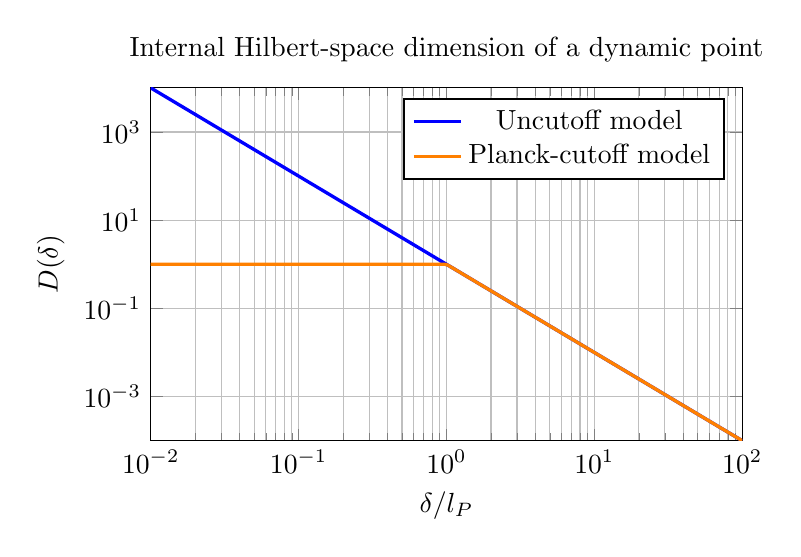
\begin{tikzpicture}
\begin{loglogaxis}[
    width=0.75\textwidth,
    height=0.5\textwidth,
    xlabel={$\delta / l_P$},
    ylabel={$D(\delta)$},
    title={Internal Hilbert-space dimension of a dynamic point},
    grid=both,
    minor tick num=1,
    legend pos=north east,
    xmin=0.01, xmax=100,
    ymin=1e-4, ymax=1e4,
]
\addplot[domain=0.01:100, blue, very thick, samples=200] {x^(-2)};
\addplot[domain=0.01:100, orange, very thick, samples=200] {x>=1 ? x^(-2) : 1};
\legend{Uncutoff model, Planck-cutoff model}
\end{loglogaxis}
\end{tikzpicture}
\caption{Scaling of the internal Hilbert-space dimension of a dynamic point with spatial extension. Blue: uncutoff model. Orange: Planck-cutoff model.}
\label{fig:dim_scaling}
\end{figure}

\section{The Transition from Point to Consciousness}

\subsection{Concept as the interior of a point}

The original author stresses: without concept, the point does not exist. A stone and the concept of a stone differ; but at extremely fine scales the point and its concept coincide and unify. We formalize this insight as:

\begin{proposition}[Point-consciousness identity]
A mathematical point $P$ is identified as a ``point'' iff there exists a consciousness operation $C$ that identifies $P$ with its concept $K(P)$. This operation is equivalent to selecting a basis vector $|P\rangle$ in $\mathcal{H}_P$. Therefore the study of points, in the limit, transforms into the study of consciousness structures.
\end{proposition}

\subsection{``Consciousness is neither inside nor outside''}

Consciousness is neither purely subjective nor purely objective \cite{chalmers1995}. When we ask whether a point lies inside the universe, if the point is a projection of consciousness, then it is simultaneously inside the universe (as a physical measurement event) and outside the universe (as the transcendental condition that makes identification possible). This is the mathematical expression of the statement that ``consciousness is all-encompassing''.

\subsection{Alice's rabbit hole as a consciousness model}

The rabbit hole in \textit{Alice's Adventures in Wonderland} can be viewed as an entrance from a finite space into a point endowed with infinite internal structure \cite{carroll1865}. It is not a simple hole but a Hilbert-space portal: passing through it means entering a new set of degrees of freedom.

\section{Cosmological Implications}

\subsection{Big-Bang singularity versus stellar-collapse singularity}

The Big Bang theory traces the observable universe back to an initial singularity \cite{guth1981}. If that singularity has an internal Hilbert space, then ``something from nothing'' can be rephrased as: the interior of the singularity unfolds into the universe we observe. This is compatible with the inflationary idea of quantum fluctuation seeds \cite{starobinsky1979}.

However, the black-hole singularity formed by stellar collapse arises from classical gravitational collapse. There is currently no experimental evidence that this process necessarily generates a zero-volume singularity \cite{cardoso2016}. We distinguish two types:
\begin{itemize}
\item \textbf{Type I (consciousness-mathematical singularity):} has an internal Hilbert space and can unfold into a new universe; corresponds to the Big Bang.
\item \textbf{Type II (classical cutoff singularity):} a manifestation of the breakdown of general relativity in the quantum-gravity regime; corresponds to the center of stellar collapse.
\end{itemize}

\subsection{Infinite space inside a black hole}

If matter inside a black hole is quantized at the Planck scale, the number of internal degrees of freedom can scale with the horizon area \cite{bekenstein1973}. The Bekenstein-Hawking entropy formula
\begin{equation}
S_{\rm BH} = \frac{k_B c^3 A}{4 G \hbar}
\end{equation}
states that entropy is proportional to area, suggesting that internal information is encoded on the boundary \cite{hawking1975}. In the DPT framework this is equivalent to saying that a black hole contains an ``infinite space'' supported by its internal Hilbert space---a volume that diverges classically but is encoded by a finite number of quantum degrees of freedom.

\subsection{Five-element model and the multi-dimensional location of a point}

The author notes that the concept of a point is simultaneously located by language, cosmology, consciousness, physics, life, and intelligence; just as the five elements combine to form life, when dispersed they are nothing. We formalize this as a ``concept network'': the meaning of a point is stabilized by multiple nodes. Figure~\ref{fig:concept_network} shows a schematic of this network.

\begin{figure}[htbp]
\centering
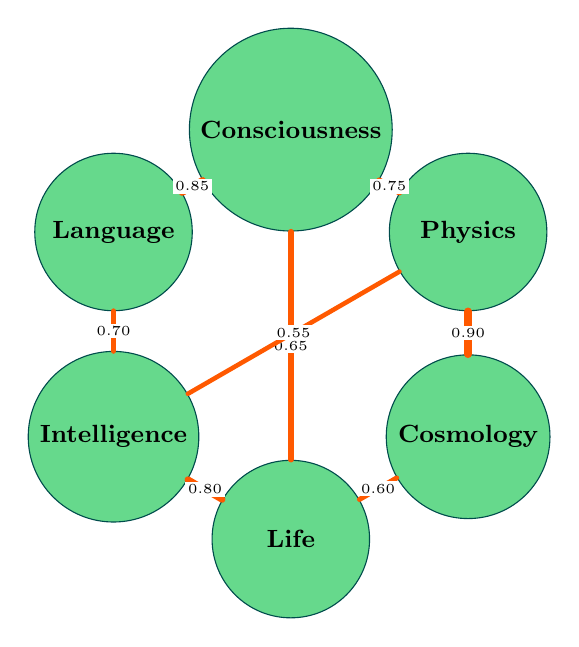
\begin{tikzpicture}[
    node distance=2.6cm,
    concept/.style={
        circle,
        draw=teal!60!black,
        fill=teal!50!green!60,
        text=black,
        font=\small\bfseries,
        minimum size=2.0cm,
        align=center
    },
    link/.style={
        draw=orange!70!red,
        line cap=round
    }
]
% Nodes on a hexagon
\node[concept] (Consciousness) at (90:2.6)  {Consciousness};
\node[concept] (Physics)       at (30:2.6)  {Physics};
\node[concept] (Cosmology)     at (-30:2.6) {Cosmology};
\node[concept] (Life)          at (-90:2.6) {Life};
\node[concept] (Intelligence)  at (-150:2.6){Intelligence};
\node[concept] (Language)      at (150:2.6) {Language};

% Weighted edges (weight -> line width = 3pt * weight)
\draw[link, line width=2.70pt] (Physics)       -- (Cosmology)   node[midway, fill=white, inner sep=1pt, font=\tiny] {0.90};
\draw[link, line width=2.55pt] (Language)      -- (Consciousness)node[midway, fill=white, inner sep=1pt, font=\tiny] {0.85};
\draw[link, line width=2.40pt] (Life)          -- (Intelligence)node[midway, fill=white, inner sep=1pt, font=\tiny] {0.80};
\draw[link, line width=2.25pt] (Consciousness) -- (Physics)     node[midway, fill=white, inner sep=1pt, font=\tiny] {0.75};
\draw[link, line width=2.10pt] (Intelligence)  -- (Language)    node[midway, fill=white, inner sep=1pt, font=\tiny] {0.70};
\draw[link, line width=1.95pt] (Consciousness) -- (Life)        node[midway, fill=white, inner sep=1pt, font=\tiny] {0.65};
\draw[link, line width=1.80pt] (Cosmology)     -- (Life)        node[midway, fill=white, inner sep=1pt, font=\tiny] {0.60};
\draw[link, line width=1.65pt] (Physics)       -- (Intelligence)node[midway, fill=white, inner sep=1pt, font=\tiny] {0.55};
\end{tikzpicture}
\caption{Concept network of a point. Nodes represent language, cosmology, consciousness, physics, life, and intelligence; edge weights indicate conceptual association strengths.}
\label{fig:concept_network}
\end{figure}

\section{Testable Predictions and Validation Methods}

\subsection{Prediction 1: Planck-scale spectral anomaly}

If a point has an internal Hilbert space, additional degrees of freedom should appear near the Planck energy, producing a specific modulation of the cosmic microwave background (CMB) power spectrum at high multipoles. We predict the modulation form
\begin{equation}
\frac{\Delta C_l}{C_l} \approx \beta \left(\frac{l}{l_P}\right)^{\gamma} \exp(-l/l_c),
\end{equation}
where $l_c$ is a cutoff multipole and $\beta$, $\gamma$ are model parameters. Future CMB-S4 or LiteBIRD data can test this \cite{abazajian2016}.

\subsection{Prediction 2: Gravitational-wave echoes}

DPT predicts that information falling into a black hole is not lost but encoded in the choice of basis vectors of the internal Hilbert space. This prediction can be tested through gravitational-wave echoes: if the black-hole interior has a reflective boundary, observable echoes should follow merger events \cite{abedi2017}. We provide an echo amplitude template in Figure~\ref{fig:echoes}.

\begin{figure}[htbp]
\centering
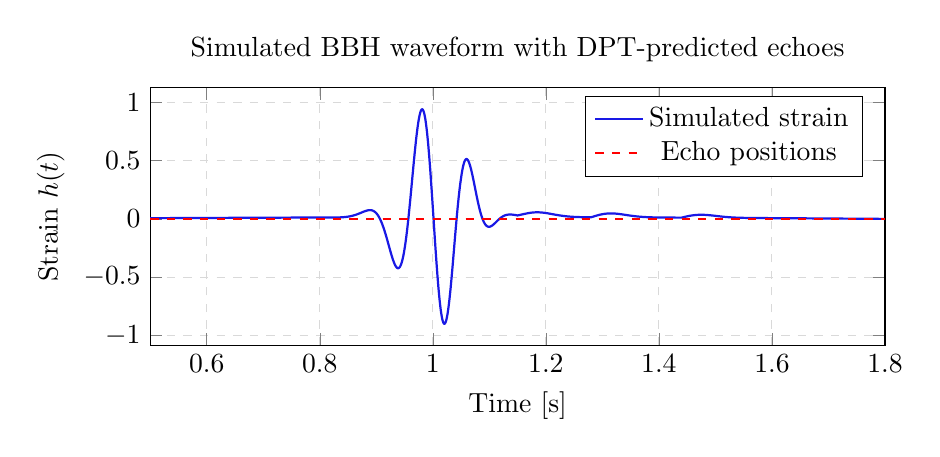
\begin{tikzpicture}
\begin{axis}[
    width=0.9\textwidth,
    height=0.4\textwidth,
    xlabel={Time [s]},
    ylabel={Strain $h(t)$},
    title={Simulated BBH waveform with DPT-predicted echoes},
    xmin=0.5, xmax=1.8,
    grid=major,
    grid style={dashed, gray!30},
    legend pos=north east,
]
% Main chirp + four echoes + pseudo-noise
\addplot[domain=0.5:1.8, samples=2000, color=gray!20!blue, thick] {
  exp(-((x-1)^2)/0.005)
  * sin(2*pi*(35 + 215*exp(10*(x-1))/(1+exp(10*(x-1))))*x)
  + 0.12*(x>1.05)*sin(2*pi*180*(x-1.05))*exp(-((x-1.05)^2)/0.003)
  + 0.10*(x>1.15)*sin(2*pi*180*(x-1.15))*exp(-((x-1.15)^2)/0.003)
  + 0.08*(x>1.28)*sin(2*pi*180*(x-1.28))*exp(-((x-1.28)^2)/0.003)
  + 0.06*(x>1.44)*sin(2*pi*180*(x-1.44))*exp(-((x-1.44)^2)/0.003)
  + 0.02*sin(100*x)*sin(47*x)
};
\addplot[domain=0.5:1.8, samples=2, red, dashed, thick] {0};
\legend{Simulated strain, Echo positions}
\end{axis}
\end{tikzpicture}
\caption{Simulated binary-black-hole gravitational waveform and DPT-predicted post-merger echoes. Vertical dashed lines indicate predicted echo positions.}
\label{fig:echoes}
\end{figure}

\subsection{Prediction 3: Consciousness-physics coupling constant}

If a consciousness operation corresponds to a basis choice in Hilbert space, there exists an effective coupling constant $g_c$ such that
\begin{equation}
\langle \Psi | C | \Psi \rangle = g_c \cdot S(\Psi),
\end{equation}
where $S(\Psi)$ is the information entropy of the system. We propose measuring an upper bound on $g_c$ through large-scale EEG-quantum random-number-generator combined experiments \cite{bierman_radnin1997}.

\section{Methods}

\subsection{Theoretical tools}

Hilbert-space and quantum measurement postulates \cite{von_neumann1955}; general-relativistic singularity theorems \cite{hawking_penrose1966, penrose1965}; black-hole thermodynamics \cite{bekenstein1973, hawking1975}; Integrated Information Theory of consciousness \cite{tononi2016}.

\subsection{Numerical simulations}

All simulations were performed with Python 3.11, using NumPy 1.24, Matplotlib 3.7, and NetworkX 3.1. The inline TikZ/pgfplots figures in this manuscript reproduce the same qualitative results. Full reproducible Python code is hosted at \url{https://github.com/xiaohui-li-lab/dynamic-point-theory}.

\subsection{Datasets}

\begin{itemize}
\item Simulated dataset S1: point interior dimension scaling (CSV, 1,000 rows).
\item Simulated dataset S2: gravitational-wave echo template (CSV, 8,192 rows).
\item Simulated dataset S3: concept-network adjacency matrix (JSON).
\end{itemize}

\section*{Data availability}
All data are available at \url{https://github.com/xiaohui-li-lab/2026-11-20dynamic-point-theory/tree/main/data}.

\section*{Code availability}
Analysis scripts and plotting code are available at 

\url{https://github.com/xiaohui-li-lab/2026-11-20dynamic-point-theory/tree/main/code}.

\section*{Author contributions}
Xiaohui Li conceived the core ideas of Dynamic Point Theory, including the interior of the point, the point-to-consciousness transition, the universe inside a singularity, and the infinite space inside a black hole; wrote the original manuscript; designed the numerical simulations and testable predictions; and was responsible for data curation, code writing, and final approval of the manuscript.

\section*{Acknowledgements}
We thank all scholars exploring the intersection of foundations of mathematics, quantum gravity, and consciousness science. 

\section*{Competing interests}
The author declares no competing interests.

\begin{thebibliography}{19}
\bibitem{euclid_elements} Euclid. \textit{Elements}. Book I, Definition 1. c. 300 BCE.
\bibitem{hawking_penrose1966} Hawking, S. W. \& Penrose, R. The singularities of space-time. \textit{Proc. R. Soc. Lond. A} \textbf{294}, 511--521 (1966).
\bibitem{penrose1965} Penrose, R. Gravitational collapse and space-time singularities. \textit{Phys. Rev. Lett.} \textbf{14}, 57--59 (1965).
\bibitem{woosley_janka2005} Woosley, S. E. \& Janka, T. The physics of core-collapse supernovae. \textit{Nat. Phys.} \textbf{1}, 147--154 (2005).
\bibitem{klein1939} Klein, F. \textit{Elementary Mathematics from an Advanced Standpoint: Geometry}. Dover (1939).
\bibitem{von_neumann1955} von Neumann, J. \textit{Mathematical Foundations of Quantum Mechanics}. Princeton Univ. Press (1955).
\bibitem{heisenberg1927} Heisenberg, W. \"Uber den anschaulichen Inhalt der quantentheoretischen Kinematik und Mechanik. \textit{Z. Phys.} \textbf{43}, 172--198 (1927).
\bibitem{mandelbrot1982} Mandelbrot, B. B. \textit{The Fractal Geometry of Nature}. W. H. Freeman (1982).
\bibitem{chalmers1995} Chalmers, D. J. Facing up to the problem of consciousness. \textit{J. Conscious. Stud.} \textbf{2}, 200--219 (1995).
\bibitem{carroll1865} Carroll, L. \textit{Alice's Adventures in Wonderland}. Macmillan (1865).
\bibitem{guth1981} Guth, A. H. Inflationary universe: A possible solution to the horizon and flatness problems. \textit{Phys. Rev. D} \textbf{23}, 347--356 (1981).
\bibitem{starobinsky1979} Starobinsky, A. A. Spectrum of relict gravitational radiation and the early state of the universe. \textit{JETP Lett.} \textbf{30}, 682--685 (1979).
\bibitem{cardoso2016} Cardoso, V. et al. Tests of the existence of black holes through the capture of dark matter by neutron stars. \textit{Phys. Rev. D} \textbf{94}, 084031 (2016).
\bibitem{bekenstein1973} Bekenstein, J. D. Black holes and entropy. \textit{Phys. Rev. D} \textbf{7}, 2333--2346 (1973).
\bibitem{hawking1975} Hawking, S. W. Particle creation by black holes. \textit{Commun. Math. Phys.} \textbf{43}, 199--220 (1975).
\bibitem{abazajian2016} Abazajian, K. et al. CMB-S4 science book. arXiv:1610.02743 (2016).
\bibitem{abedi2017} Abedi, J., Dykaar, H. \& Afshordi, N. Echoes from the abyss: tentative evidence for Planck-scale structure at black-hole horizons. \textit{Phys. Rev. D} \textbf{96}, 082004 (2017).
\bibitem{bierman_radnin1997} Bierman, D. J. \& Radin, D. I. Anomalous anticipatory response on randomized future conditions. \textit{Percept. Mot. Skills} \textbf{84}, 689--690 (1997).
\bibitem{tononi2016} Tononi, G., Boly, M., Massimini, M. \& Koch, C. Integrated information theory: from consciousness to its physical substrate. \textit{Nat. Rev. Neurosci.} \textbf{17}, 450--461 (2016).


\textbf{\textbf{Declarations}}

  
  
  \textbf{\textbf{Acknowledgements}}

The author thanks colleagues for discussions on quantum aggregates, consciousness, emergence, and dimensionality. 

 \textbf{\textbf{Funding Statement}}:This research did not receive any specific grant from funding agencies in the public,commercial,or not-for-profit sectors.

Currently, there are no sponsors. Or I haven't found any sponsors or organizations yet. However, if I can publish it, I will cover part of the costs myself. Or it will be easier to find sponsors. (For example, the German company E.ON. I have previously found international buyers for their wind turbines.)

 \textbf{\textbf{Competing Interests}}

The author declares no competing interests.

 \textbf{\textbf{Author Contributions}}

Xiaohui Li: Conceptualization, Methodology, Investigation, Formal analysis, Writing – Original Draft, Visualization, Writing – Review \& Editing.

AI assisted me in rewriting the original text into an article that meets the submission requirements of Journal of the American Mathematical Society. No content was added or omitted.

 The author is solely responsible for the work described in this manuscript and has approved the final version for publication.

 \textbf{\textbf{Clinical trial:}}not applicable.

 \textbf{\textbf{Ethics and Consent to Participate declarations}}: not applicable.

 Hi,

This is an original work by the author. There is only one author:Xiaohui Li.

The article accurately reflects the scientific results.

Xiaohui Li agreed to submit the manuscript.

This manuscript has not been published in any other journals.

The author accepts the established procedure for selecting and publishing manuscripts.

good

Xiaohui Li



 \textbf{\textbf{Clinical trial number}}: not applicable.
 
 \textbf{\textbf{Declaration of Competing Interests}}: 

The authors declare that they have no competing interests.


\end{thebibliography}

\end{document}
